% Перестроение в двумерном случае.
\subsection{Методы перестроения поверхности в двумерном случае}

Рассмотрим геометрическую задачу о перестроении поверхности в двумерном пространстве в общем виде \cite{Rybakov2019Geo2D}.
Пусть даны $n$ ячеек поверхностной сетки, каждая из которых представлена отрезком длины $l_i$ (то есть общее количество узлов равно $n + 1$).
Известно направление нормали каждой ячейки, а также направление движения каждого узла $\overline{g_i}$, $|\overline{g_i}| = 1$.
Оно совпадает с направлением суммы единичных нормалей, проведенных к инцидентным ячейкам.
К тому же для двумерного случая это направление лежит на биссектрисе угла, образованного двумя инцидентными ячейками \cite{Fortin2004Remesh2d} (рис.~\ref{fig:text_1_remesh_2d_grid_normals}).

\begin{figure}[h]
\centering
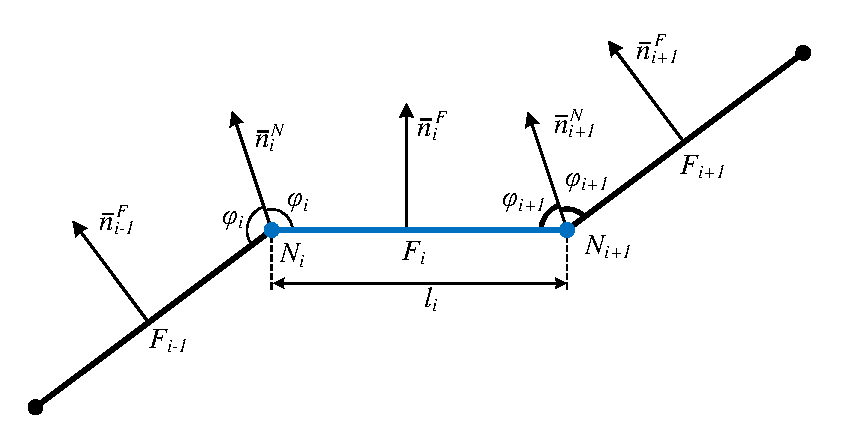
\includegraphics[width=0.7\textwidth]{pics/text_1_remesh_2d/grid_normals.pdf}
\singlespacing
\captionstyle{center}\caption{Поверхностная сетка с обозначенными направлениями движения узлов.}
\label{fig:text_1_remesh_2d_grid_normals}
\end{figure}

Пусть известно, что за некий малый промежуток времени $i$-ая ячейка сдвигается в направлении своей нормали на малую величину $H_i$, заметая таким образом площадь $T_i = l_i H_i$.
Но если просто сдвинуть каждую ячейку в направлении своей нормали, то сетка потеряет целостность, поэтому мы можем осуществлять движение только узлов.
Требуется найти такие значения локальных сдвигов узлов сетки $h_i$, чтобы заметаемая площадь между исходной поверхностью и новой поверхностью для каждой ячейки сетки ($S_i$) как можно меньше отличалась от требуемого значения $T_i = l_iH_i$.

Для решения данной задачи сначала требуется вычислить заметаемую площадь для каждой отдельной ячейки.

\subsubsection{Задача о вычислении заметаемой площади при движении узлов отдельной ячейки}

Рассматривается ячейка, представленная на плоскости отрезком $AB$ длины $l$.
При перемещении точек $A$ и $B$ в новые точки $A_1$ и $B_1$ соответственно образуется четырехугольник $AA_1B_1B$.
Требуется найти его площадь, выраженную явно через параметры $a = \overline{AA_1}$ и $b = \overline{BB_1}$ (рис.~\ref{fig:text_1_remesh_2d_local}).

\begin{figure}[h]
\centering
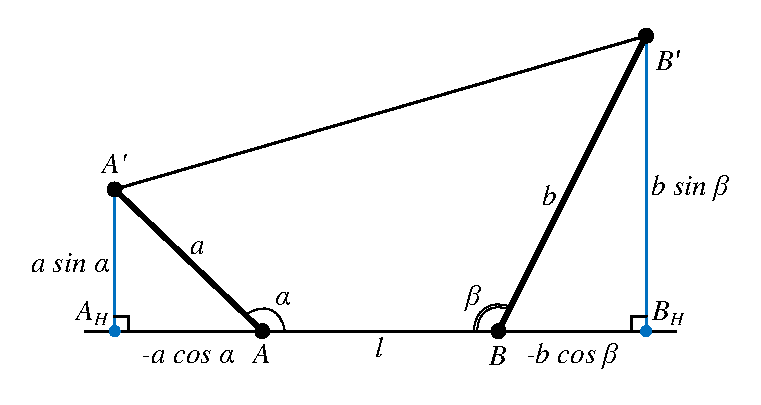
\includegraphics[width=0.7\textwidth]{pics/text_1_remesh_2d/local.pdf}
\singlespacing
\captionstyle{center}\caption{Вычисление заметаемой площади через смещения узлов ячейки.}
\label{fig:text_1_remesh_2d_local}
\end{figure}

Для решения задачи опустим перпендикуляры из точек $A_1$ и $B_1$ на прямую $AB$.
Их основаниями будут точки $A_2$ и $B_2$ соответственно.
Искомая площадь может быть представлена в следующем виде:
\begin{equation}
S_{AA_1B_1B} = S_{A_2A_1B_1B_2} - S_{AA_1A_2} - S_{BB_1B_2}
\end{equation}

Обозначим угол между векторами $\overline{AA_1}$ и $\overline{AB}$ через $\alpha$, а угол между векторами $\overline{BB_1}$ и $\overline{BA}$ через $\beta$.
Тогда искомая площадь вычисляется явно в следующем виде:
\begin{equation}
S_{AA_1B_1B} = \frac{1}{2}(l - a \cos \alpha - b \cos \beta)(a \sin \alpha + b \sin \beta) + \frac{1}{2}a^2 \sin \alpha \cos \alpha + \frac{1}{2}b^2 \sin \beta \cos \beta
\end{equation}

\begin{equation}\label{eqn:text_1_remesh2_loca_square}
S_{AA_1B_1B} = \frac{1}{2}\big(l(a \sin \alpha + b \sin \beta) - ab \sin(\alpha + \beta)\big)
\end{equation}

Формула \eqref{eqn:text_1_remesh2_loca_square} применима как для значений $\alpha \ge \frac{\pi}{2}$, $\beta \ge \frac{\pi}{2}$ (это случай изображен на рис.~\ref{fig:text_1_remesh_2d_local}), так и для $\alpha < \frac{\pi}{2}$, $\beta < \frac{\pi}{2}$.
Ограничение применения формулы \eqref{eqn:text_1_remesh2_loca_square} наступает, когда значение площади $S_{AA_1B_1B}$ перестает расти при возрастании $a$ и $b$, то есть при условиях
\begin{equation}
	\begin{aligned}
		\frac{\partial S_{AA_1B_1B}}{\partial a} = \frac{1}{2}(l \sin \alpha - b \sin (\alpha + \beta)) = 0 \\
		\frac{\partial S_{AA_1B_1B}}{\partial b} = \frac{1}{2}(l \sin \beta - a \sin (\alpha + \beta)) = 0
	\end{aligned}
\end{equation}

откуда получаем
\begin{equation}
	\begin{aligned}
		a = \frac{l \sin \beta}{\sin (\alpha + \beta)} \\
		b = \frac{l \sin \alpha}{\sin (\alpha + \beta)}
	\end{aligned}
\end{equation}

что соответствует ситуации, когда точки $A_1$ и $B_1$ слились в одну и образовался треугольник со сторонами $a$, $b$, $l$.
Эта ситуация означает возникновение самопересечения сетки, которое должно быть обработано отдельно для возможности продолжения работы с расчетной сеткой.

\subsubsection{Поиск смещений узлов методом градиентного спуска}

Метод градиентного спуска является одним из наиболее простых методом оптимизации для нахождения локального минимума функции.
При условии, что в любой точке функции можно вычислить ее градиент, то начиная с некоторого начального приближения $x_0$ строится итерационная последовательность~\cite{Kantorovich1984Func}:
\begin{equation}
x^{k+1} = x^k - \gamma_k \nabla f(x_k)
\end{equation}

где $\gamma_k \ge 0$ задает длину шага и, соответственно, скорость градиентного спуска.

Градиентный метод находит свое основное применение в задаче поиска минимума или максимума функции.
Направление антиградиента является направлением наискорейшего убывания функции.
Основная проблема метода заключается в выборе шага $\gamma$.
При слишком больших значениях шага существует вероятность миновать искомый минимум функции.
К тому же, метод не гарантирует нахождение глобального минимума.

Рассмотрим решение задачи определения величин смещения узлов расчетной сетки при перестроении методом градиентного спуска.
Неизвестными параметрами являются величины сдвигов узлов сетки $h_i$ для $0 \le i \le n$.
Опираясь на решение локальной задачи об определении заметаемой площади, можно записать заметаемую площадь при движении отдельной ячейки:
\begin{equation}
S_i = \frac{1}{2}\big(l_i(h_i \sin \alpha_i + h_{i + 1} \sin \beta_i) - h_ih_{i + 1} \sin(\alpha_i + \beta_i)\big) 
\end{equation}

Отклонением охватываемой площади в ячейке от истинного значения будем называть величину $\delta_i = S_i - T_i$, а ошибкой -- ее квадрат $d_i = \delta_i^2$.
Общая ошибка при перестроении поверхности задается как сумма ошибок для всех ячеек:
\begin{equation}
D = \sum_{i = 0}^{n - 1}{d_i}
\end{equation}

При нахождении оптимального решения требуется минимизировать общую ошибку.
Для нахождения градиента требуется вычислить частные производные функции $D$ по всем неизвестным $h_i$.
Эти частные производные можно записать в явном виде:
\begin{equation}
\frac{\partial D}{\partial h_i} = \frac{\partial d_{i - 1}}{\partial h_i} + \frac{\partial d_i}{\partial h_i}
\end{equation}

где
\begin{equation}
\begin{cases}
\frac{\partial d_{i - 1}}{\partial h_i} = \delta_{i - 1}(l_{i - 1} \sin \beta_{i - 1} - h_{i - 1} \sin(\alpha_{i - 1} + \beta_{i - 1})) \\
\frac{\partial d_i}{\partial h_i} = \delta_i(l_i \sin \alpha_i - h_{i + 1} \sin(\alpha_i + \beta_i))
\end{cases}
\end{equation}

\

Также при осуществлении метода градиентного спуска требуется следить за соблюдением дополнительных условий, которые накладываются на неизвестные $h_i$.
Например, очевидным условием является выполнение соотношения $h_i \ge 0$, что запрещает движение сетки в отрицательном направлении.
В нашем случае использовались более строгие условия $\min(H_{i - 1}, H_i) \le h_i \le \max(H_{i - 1}, H_i)$, которые не позволят величинам смещения узлов сетки выходить за пределы смещений инцидентных им ячеек сетки.

\subsubsection{Приближенные методы перестроения поверхности}

Решение задачи о перестроении сетки методом градиентного спуска оказывается слишком требовательным к ресурсам при увеличении размера сетки.
К тому же, качество решения зачастую оказывается неудовлетворительным, особенно при попадании в локальные минимумы.
Поэтому для решения поставленной задачи рассмотрим приближенные методы, основанные на представлении охватываемой площади при движении каждой ячейки с помощью примитивных геометрических фигур.

В качестве первого метода рассмотрим приближение, при котором каждый узел сетки сдвигается на вектор $\frac{1}{2}(H_{i - 1} + H_i)\overline{g_i}$.
Этот метод соответствует представлению площади, охватываемой при движении ячейки длины $l_i$, прямоугольником cо сторонами $l_i$ и $H_i$, а затем выбору в качестве величины смещения узла среднего арифметического высот построенных прямоугольников в инцидентных ячейках, как показано на рис.~\ref{fig:text_1_remesh_2d_grid_rectangles}.

\begin{figure}[h]
\centering
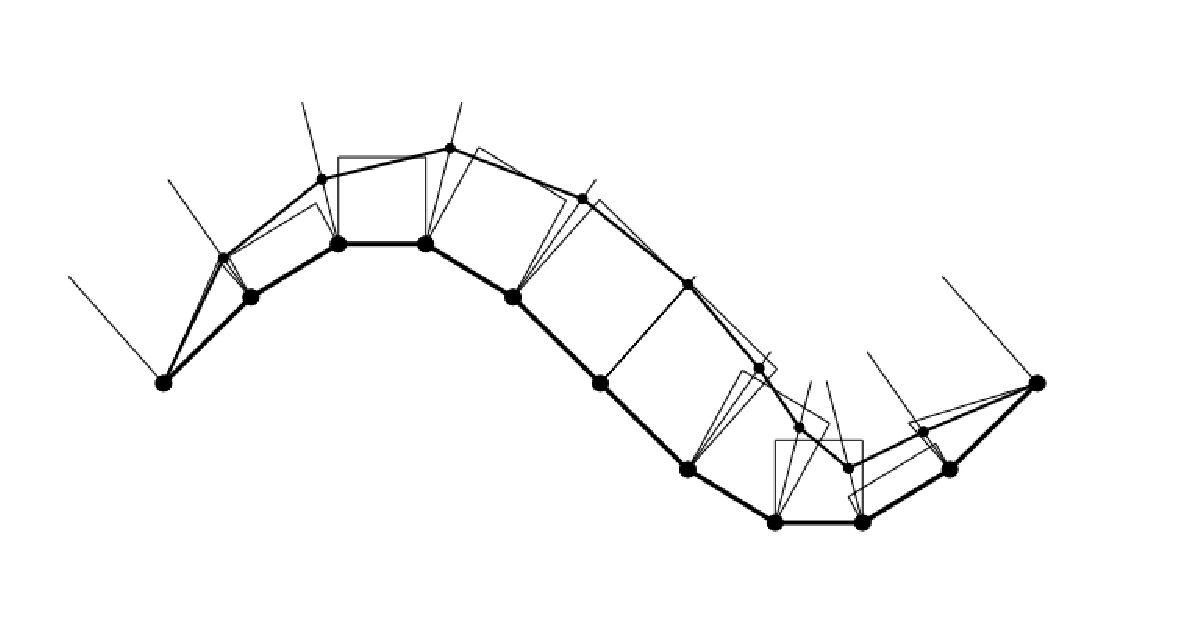
\includegraphics[width=0.7\textwidth]{pics/text_1_remesh_2d/grid_rectangles.pdf}
\singlespacing
\captionstyle{center}\caption{Перестроение поверхности методом прямоугольников.}
\label{fig:text_1_remesh_2d_grid_rectangles}
\end{figure}

В методе трапеций охватываемая площадь при движении ячейки представляется трапецией с площадью $T_i$, боковые стороны которой лежат на направлениях движения двух узлов, относящихся к рассматриваемой ячейке (направения $\overline{g}_{i - 1}$, $\overline{g}_i$).
После построения трапеций для всех ячеек сетки у каждого внутреннего узла появляется две новые потенциальные позиции для сдвига (образованные ячейкой слева и ячейкой справа).
В качестве финальной новой позиции выбирается их среднее значение (рис.~\ref{fig:text_1_remesh_2d_grid_trapeziums}).

\begin{figure}[h]
\centering
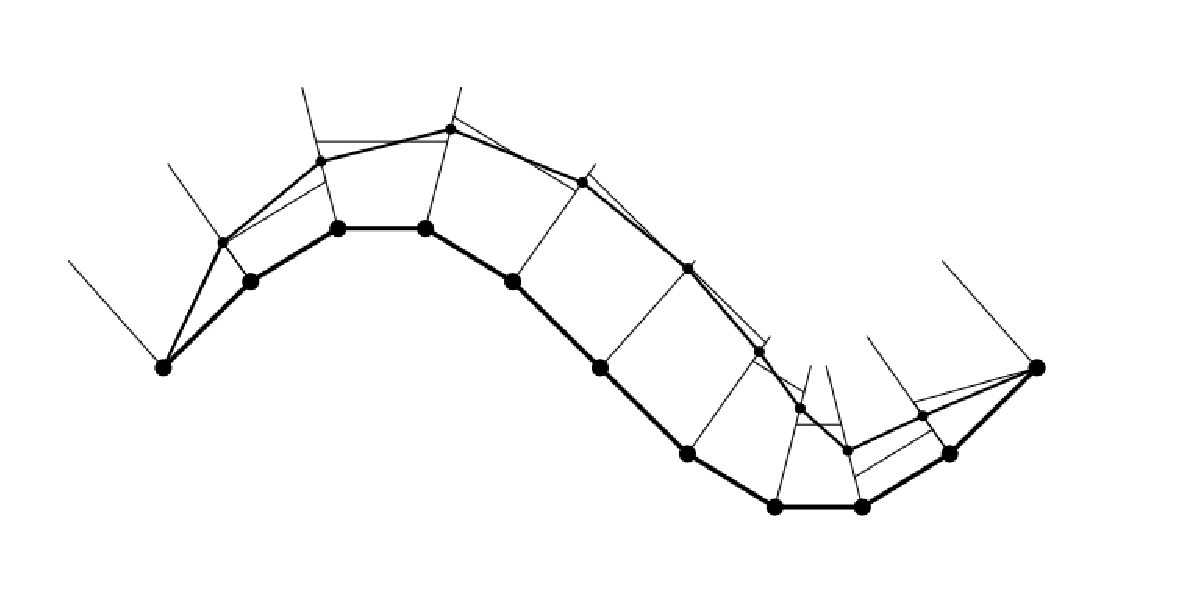
\includegraphics[width=0.7\textwidth]{pics/text_1_remesh_2d/grid_trapeziums.pdf}
\singlespacing
\captionstyle{center}\caption{Перестроение поверхности методом трапеций.}
\label{fig:text_1_remesh_2d_grid_trapeziums}
\end{figure}

Приведем теоретическую оценку точности приближенных методов перестроения поверхности.
Оценку будем проводить для модельной расчетной сетки, которая удовлетворяет следующим требованиям.
Все ячейки сетки одинаковые и имеют длину $l$, поверхность является выпуклой.
Для любой ячейки $AB$ и ее соседей $A_1A$ и $BB_1$ углы $\angle (\overline{BA}, \overline{AA_1})$ и $\angle (\overline{AB}, \overline{BB_1})$ являются постоянной величиной и равны $\alpha$ (см. рис.~\ref{fig:text_1_remesh_2d_theoretical}).
Пусть величины смещений ячеек $A_1A$, $AB$ и $BB_1$ равны $H^{-}$, $H$ и $H^{+}$ соответственно.

\begin{figure}[h]
\centering
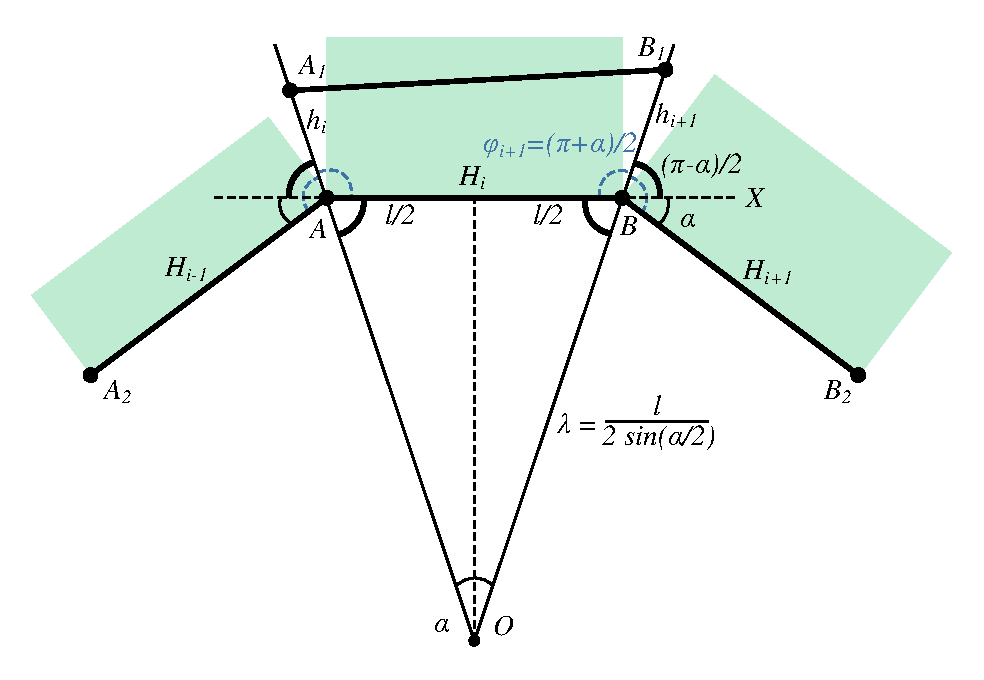
\includegraphics[width=0.8\textwidth]{pics/text_1_remesh_2d/theoretical.pdf}
\singlespacing
\captionstyle{center}\caption{Теоретическая оценка приближенных методов перестроения выпуклой поверхности в двумерном случае.}
\label{fig:text_1_remesh_2d_theoretical}
\end{figure}

Отклонение от требуемой площади при использовании приближенных методов перестроения поверхности равно $\delta = S_{AA_2B_2B} - lH$.
Относительное отклонение будем обозначать через $\breve{\delta} = \frac{\delta}{lH}$.
Для вычисления отклонения необходимо вычислить площадь $S_{AA_2B_2B}$.
При использовании разных методов перестроения эта площадь будет различаться, для метода прямоугольников обозначим ее через $S_{AA_2B_2B}^r$, а для метода трапеций -- через $S_{AA_2B_2B}^t$.

Пусть в результате перестроения узлы $A$ и $B$ сместились в новые положения $A_2$ и $B_2$ соответственно ($AA_2 = h^{-}$, $BB_2 = h^{+}$).
Так как мы рассматриваем выпуклую сетку то лучи $A_2A$ и $B_2B$ пересекаются в некоторой точке $O$.
При этом треугольник $AOB$ равнобедренный, $\angle BAO = \angle ABO = \angle B_2BX = \angle B_2BB_1 - \alpha = \frac{\pi - \alpha}{2}$, $\angle AOB = \alpha$, откуда $OA = OB = \lambda = \frac{l}{2 \sin \frac{\alpha}{2}}$.
Далее можно выразить площадь $S_{AA_2B_2B} = S_{A_2OB_2} - S_{AOB}$:
\begin{equation}\label{eqn:text_1_remesh2_saa2b2b_gen}
	S_{AA_2B_2B} = \frac{1}{2} \sin \alpha \left( \lambda(h^{-} + h^{+}) + h^{-}h^{+} \right)
\end{equation}

Далее будем рассматривать линейное изменение величины смещения ячеек сетки, то есть $H^{-} = H - \Delta H$, $H^{+} = H + \Delta H$.

Для перестроения методом прямоугольников имеем $h^{-} = H - \frac{1}{2} \Delta H$, $h^{+} = H + \frac{1}{2} \Delta H$, откуда
\begin{equation}\label{eqn:text_1_remesh2_s_rect}
	S_{AA_2B_2B}^r = \cos \frac{\alpha}{2} \left( lH + \left( H^2 - \frac{1}{4} \Delta H^2 \right) \sin \frac{\alpha}{2} \right)
\end{equation}

Теперь перейдем к вычислению $S_{AA_2B_2B}^t$ для метода трапеций.
В методе трапеций мы должны представить заметаемые площади в ячейках $A_1A$, $AB$, $BB_1$ с помощью равнобоких трапеций, для которых известно одно из оснований (одинаково для всех ячеек и равно $l$), угол при другом основании (одинаковый для всех ячеек и равен $\frac{\pi - \alpha}{2}$, а также площади этих трапеций, равные $lH^{-} = l(H - \Delta H)$, $lH$ и $lH^{+} = l(H + \Delta H)$ соответственно.
На основании этих данных нам необходимо вычислить высоты трапеций, что можно сделать согласно \eqref{eqn:text_1_geo_prim_trapezium_h_from_s}.
Обозначим высоты этих трапеций:
\begin{equation}
	\begin{aligned}	
		& h_t^{A_1A} = h_t^{-} = h\left(\frac{\pi - \alpha}{2}, l, l(H - \Delta H)\right) \\ 
		& h_t^{AB} = h_t = h\left(\frac{\pi - \alpha}{2}, l, lH\right) \\
		& h_t^{BB_1} = h_t^{+} = h\left(\frac{\pi - \alpha}{2}, l, l(H + \Delta H)\right)
	\end{aligned}
\end{equation}

Тогда $h^{-} = \frac{h_t^{-} + h_t}{2 \cos \frac{\alpha}{2}}$, $h^{+} = \frac{h_t + h_t^{+}}{2 \cos \frac{\alpha}{2}}$ и выражение \eqref{eqn:text_1_remesh2_saa2b2b_gen} для $S_{AA_2B_2B}^t$ принимает следующий вид:
\begin{equation}\label{eqn:text_1_remesh2_trap}
	S_{AA_2B_2B}^t = \frac{1}{4} \left( (h_t^{-} + 2 h_t + h_t^{+})l + (h_t^{-} + h_t) (h_t + h_t^{+}) \tg \frac{\alpha}{2} \right)
\end{equation}

Теперь рассмотрим случай вогнутой сетки, представленный на рис.~\ref{fig:text_1_remesh_2d_theoretical_concave}.

\begin{figure}[h]
\centering
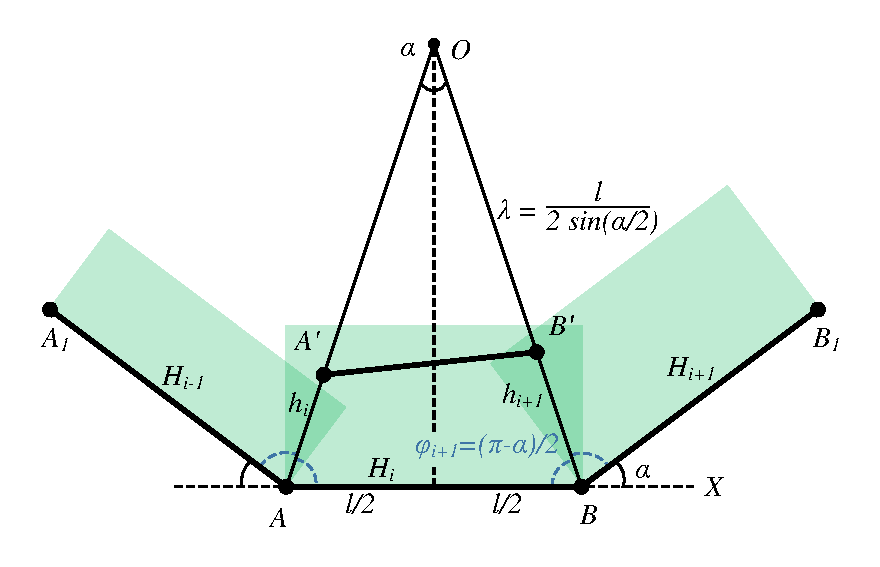
\includegraphics[width=0.8\textwidth]{pics/text_1_remesh_2d/theoretical_concave.pdf}
\singlespacing
\captionstyle{center}\caption{Теоретическая оценка приближенных методов перестроения вогнутой поверхности в двумерном случае.}
\label{fig:text_1_remesh_2d_theoretical_concave}
\end{figure}

Для общности будем рассматривать вогнутую сетку как выпуклую с параметром $\alpha < 0$.
Для вогнутой сетки вычисления производятся аналогично случаю выпуклой сетки, но при этом $\lambda = \frac{l}{2 \sin \left( -\frac{\alpha}{2} \right)}$, $S_{AA_2B_2B} = S_{AOB} - S_{A_2OB_2}$, откуда имеем
\begin{equation}\label{eqn:text_1_remesh2_concave_case}
	S_{AA_2B_2B} = \frac{1}{2} \sin (-\alpha) \left( \lambda (h^{-} + h^{+}) - h^{-} h^{+} \right)
\end{equation}

Для перестроения методом прямоугольников, подставляя $h^{-} = H - \frac{1}{2} \Delta H$, $h^{+} = H + \frac{1}{2} \Delta H$ в \eqref{eqn:text_1_remesh2_concave_case}, получим в точности \eqref{eqn:text_1_remesh2_s_rect}, что говорит о том, что \eqref{eqn:text_1_remesh2_s_rect} применима для произвольных углов $\alpha$.

Для перестроения методом трапеций аналогично подставим $h^{-} = \frac{h_t^{-} + h_t}{2 \cos\left( -\frac{\alpha}{2} \right)}$, $h^{+} = \frac{h_t + h_t^{+}}{2 \cos\left( -\frac{\alpha}{2} \right)}$ в \eqref{eqn:text_1_remesh2_concave_case} и получим в точности \eqref{eqn:text_1_remesh2_trap}, что говорит о том, что \eqref{eqn:text_1_remesh2_trap} применима для произвольных углов.

Используя \eqref{eqn:text_1_remesh2_s_rect} и \eqref{eqn:text_1_remesh2_trap} можно проанализировать зависимости величин $\breve{\delta}^r = \frac{S_{AA_2B_2B}^r - lH}{lH}$ и $\breve{\delta}^t = \frac{S_{AA_2B_2B}^t - lH}{lH}$ от $\alpha$ и $\Delta H$ (см. рис.~\ref{fig:text_1_remesh_2d_main_chart}).

\begin{figure}[h]
\centering
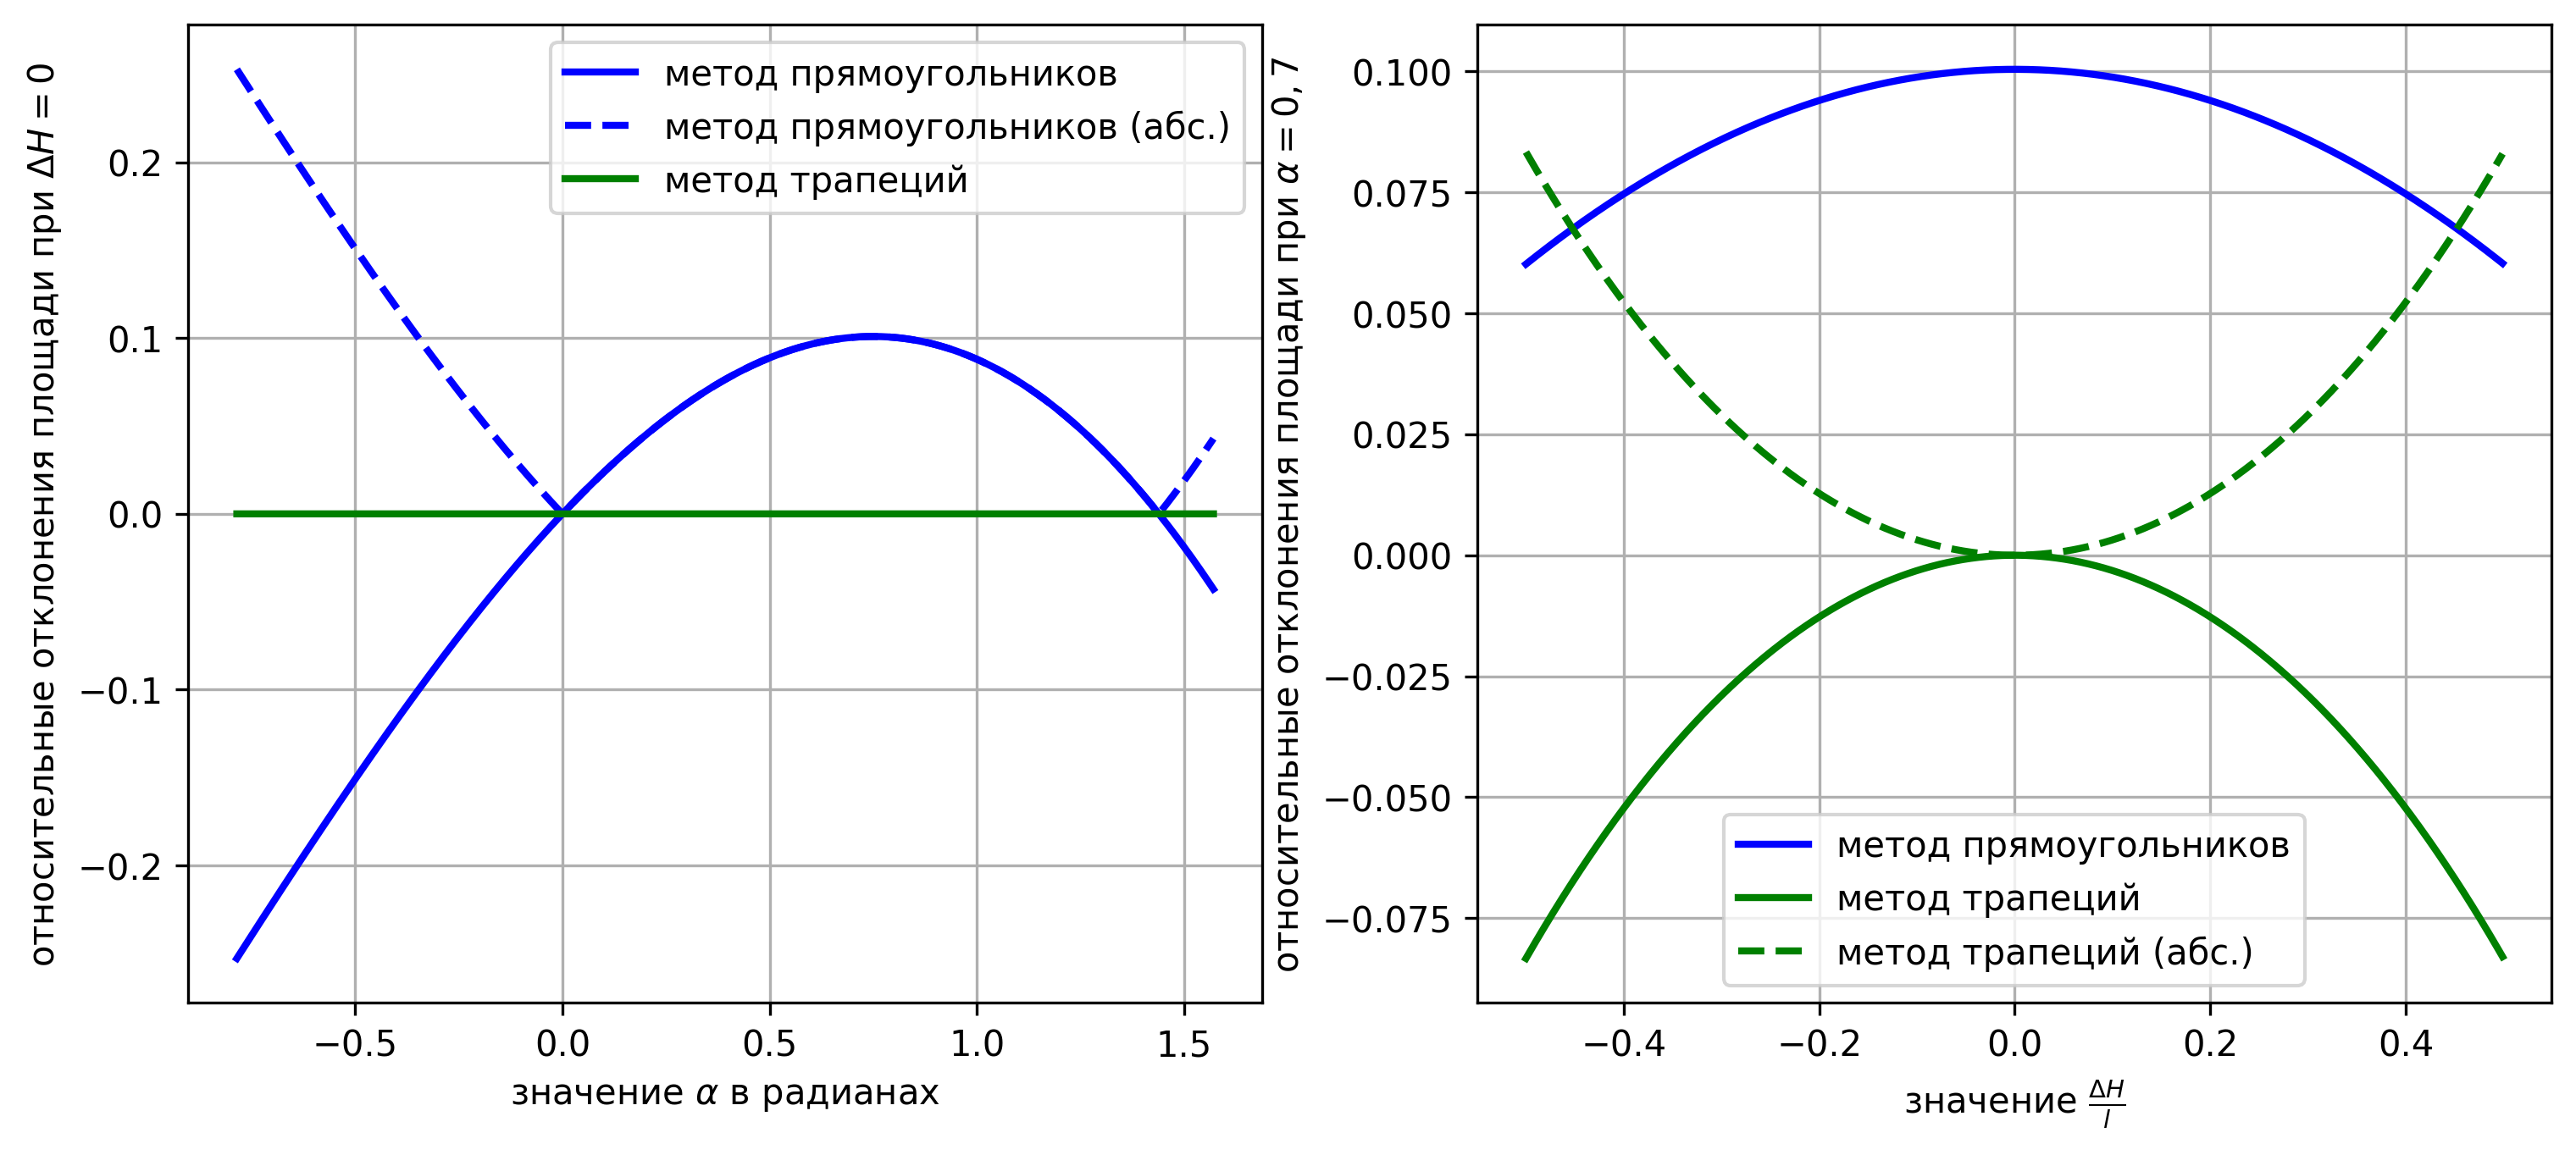
\includegraphics[width=1.0\textwidth]{pics/text_1_remesh_2d/main_chart.png}
\singlespacing
\captionstyle{center}\caption{Графики относительных отклонений заметаемых площадей $\breve{\delta}^r$ и $\breve{\delta}^t$ от целевых значений при перестроении методами прямоугольников и трапеций.}
\label{fig:text_1_remesh_2d_main_chart}
\end{figure}

На рис.~\ref{fig:text_1_remesh_2d_main_chart} слева приведены зависимости $\breve{\delta}^r$ и $\breve{\delta}^t$ от угла $\alpha$ при постоянном значении $H$, то есть при $\Delta H = 0$.
Метод трапеций в этом случае по определению абсолютно точен.
Для дальнейшего анализа было выбрано значение угла $\alpha > 0$, при котором метод прямоугольников наименее точен (это значение примерно равно 0,7) и при этом фиксированном значении $\alpha = 0,7$ были построены графики зависимостей $\breve{\delta}^r$ и $\breve{\delta}^t$ от $\Delta H$, изменяющегося в диапазоне $[-\frac{l}{2}, \frac{l}{2}]$ (см. рис.~\ref{fig:text_1_remesh_2d_main_chart} справа).
Из рисунка видно, что метод трапеций перестроения поверхности в двумерном случае более точен, чем метод прямоугольников.
